% !TeX program = pdflatex
% !BIB program = bibtex
% !BIB TS-program = bibtex
% Build references with BibTeX (or use latexmk); a biber install is not needed.
% Condensed from NSF_white_paper.tex; the original is unchanged.
% Uses the original white-paper template and refs.bib (biblatex/BibTeX).
% Figure asset: figs/fig-inverse_design_v2.2.pdf (from the original white paper).
% Review flags (not printed):
% Q1 -- AUTHOR CHECK: Specify how a local input is detected, changes the
% mechanical logic state, and affects action. Clarify whether this constitutes
% sensing, information processing, and planning under the FRR definition.
% Offline inverse design is performed by researchers, not by the robot.
% Q2 -- AUTHOR CHECK: Identify comparable existing robots and the capability
% they lack, plus a measurable improvement and experimental success criterion.
% The source supplies no benchmark; no first-of-its-kind claim is made here.
% Q3 -- SCOPE: BEAMs are the proposed experimental platform. Transferability
% to other platforms is a longer-term objective, not a demonstrated result.
% Programming refers to physical design; runtime reprogramming is not claimed.

% ----- preamble -----
% {{{
\documentclass[11pt]{article}

% page geometry, margins and figures
\usepackage{geometry}
\geometry{letterpaper, portrait, margin=0.60in}

% color and figures
\usepackage{wrapfig}
\usepackage[dvipsnames]{xcolor}
\usepackage{graphicx}

% Unused math and chemistry packages from the full template are omitted.

% font and paragraph spacing
\setlength{\parindent}{0pt} % no indent
\setlength{\parskip}{0.30\baselineskip} % adjust length a bit more; narrow = 0.25; wider = 0.34
\renewcommand{\baselinestretch}{0.95} % NSF PAPPG allows 54 lines per 9 in page (6 lines/in). 0.88 gives this.
\usepackage[T1]{fontenc}
\usepackage{lmodern} % scalable Computer Modern-style fonts
\usepackage[utf8]{inputenc}
\usepackage{microtype} % magic package that fixed the problem with my reference in the margin!!
\renewcommand{\familydefault}{\sfdefault} % for sans serif font

% --- bibliography ---
\usepackage[style=numeric-comp, eprint, backend=bibtex, doi=true,
            maxbibnames=99, sorting=none, isbn=false]{biblatex}
\renewbibmacro{in:}{}
\addbibresource{refs.bib}
\let\cite=\supercite
\AtBeginBibliography{\setlength{\emergencystretch}{1em}}

% allow reference without brackets
\DeclareCiteCommand{\citenum}
  {}
  {\printfield{labelnumber}}
  {}
  {}

% --- Compact title/authors (no affiliations) ---
\makeatletter
\renewcommand{\maketitle}{%
  \par\begingroup\centering
  {\Large\bfseries\@title\par}
  \vspace{0.35\baselineskip}
  {\normalsize\@author\par}
  \endgroup\vspace{0.6\baselineskip}}
\makeatother

% --- Format sections ---
\usepackage{titlesec}
% Reduce spacing around section/subsection titles
\titleformat{\section}{\normalfont\Large\bfseries}{\thesection}{1em}{}
\titlespacing*{\section}{0pt}{1.5ex plus 1ex minus .2ex}{0.5ex plus .2ex}
\titleformat{\subsection}{\normalfont\large\bfseries}{\thesubsection}{1em}{}
\titlespacing*{\subsection}{0pt}{1ex plus 1ex minus .2ex}{0.5ex plus .2ex}

% Caption formatting, make Figure->Fig.
\usepackage[font=small, labelfont=bf, labelsep=period, figurename=Figure]{caption} % caption formatting

% adjust bullets, list spacing to make a bit more compact
\usepackage{enumitem}
\setlist[itemize]{leftmargin=2.5ex, label=\raisebox{0.25ex}{\tiny$\bullet$}, parsep=0.25ex}

% --- Format header and footer ---
\usepackage{fancyhdr} % add/modify header & footer
\setlength{\headheight}{23pt}
\setlength{\headsep}{14pt} % fit the full header above the original text position
\pagestyle{fancy}
\fancyhf{} % sets both header and footer to nothing
\renewcommand{\headrulewidth}{0pt}
\lhead{ \small\color{gray}W{\scriptsize{}HITE} P{\scriptsize{}APER} | C{\scriptsize{}ONFIDENTIAL}\par{}}
\chead{ \small\color{gray}}
\rhead{
\includegraphics[width=5.0cm]{figs/BYUEng_Watermark.pdf}\vspace{-1ex}}
\lfoot{ \small\textcolor{gray}\today{}\par}
\rfoot{\thepage}

\date{} % no date in title, put in footnote

% --- Commenting ---
\newcommand{\rewrite}[1]{{\color{red}#1}}
\newcommand{\edit}[1]{{\color{blue}#1}}
\newcommand{\expand}[1]{{\color{purple}#1}}

\newcommand{\highlight}[1]{{\color{RoyalBlue}#1}}

%Merit Review Criteria 
%(See NSF Proposal & Award Policies & Procedures Guide, Chapter III.A.2.)
%All NSF proposals are evaluated through use of two National Science Board approved merit review criteria listed below. In some instances, however, NSF will employ additional criteria as required to highlight the specific objectives of certain programs and activities. Both criteria are to be given full consideration in the review; each criterion is necessary but neither, by itself, is sufficient.
%As a reviewer you are asked to consider what the proposers want to do, why they want to do it, how they plan to do it, how they will know if they succeed, and what benefits could accrue if the project is successful. These issues apply both to the technical aspects of the proposal and the way in which the project may make broader contributions.
%Please consider the following review elements in your review for the review criteria below:
%•	What is the potential for the proposed activity to:
%o	Advance knowledge and understanding within its own field or across different fields (Intellectual Merit); and
%o	Benefit society or advance desired societal outcomes (Broader Impacts)?
%•	To what extent do the proposed activities suggest and explore creative, original, or potentially transformative concepts?
%•	Is the plan for carrying out the proposed activities well-reasoned, well-organized, and based on a sound rationale? Does the plan incorporate a mechanism to assess success?
%•	How well qualified is the individual, team, or organization to conduct the proposed activities?
%•	Are there adequate resources available to the PI (either at the home organization or through collaborations) to carry out the proposed activities?
%Note that if additional supplementary documents are contained in the proposal, they should be reviewed as part of the Intellectual Merits and Broader Impacts, as appropriate.
% }}}

% ----- document text -----
\begin{document}

\title{A Predictive Design Framework for Programming Collective Behavior in Microrobot Swarms}
\author{Cameron K. Peterson, Douglas R. Tree, and Joseph Rich}

\maketitle
\thispagestyle{fancy}

\begin{wrapfigure}[30]{r}{2.15in}
\centering
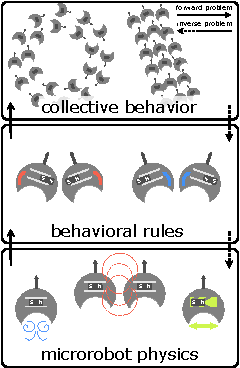
\includegraphics[width=\linewidth]{figs/fig-inverse_design_v2.2.pdf}
\caption{Proposed framework linking microrobot physics, local behavioral rules, and collective behavior. Acoustic propulsion, magnetic interactions, and mechanical logic realize local response laws. The forward problem predicts collective behavior from physical robot design through these rules; the inverse problem identifies rules and physical designs needed for a desired collective behavior.}
\label{fig:design-framework}
\end{wrapfigure}

\textbf{Opportunity and Challenge.}
Micro and nanorobotics is a growing field~\cite{Palagi2018} that promises transformative advances in medical technology,~\cite{Sun2019, Koleoso2020, Gumuskaya2023} environmental remediation,~\cite{Maria‐Hormigos2022, Urso2023, Preetam2024, Urso2022} biomimetic and dynamic materials,~\cite{Ling2018, Zhang2019, Parreira2020, Zhao2023} and many other applications.~\cite{Abdoli2022, Hecht2022, Derivaux2023}
However, microscale operation imposes severe physical and computational constraints.
%As robots decrease in size, onboard power, sensing, computation, and communication become increasingly limited.
At the same time, robots become strongly coupled to their environment and increasingly susceptible to stochastic disturbances.
Consequently, conventional robotic architectures developed for macroscale systems become fundamentally limited at the microscale.

The hardware constraints imposed at the microscale suggest that robotic intelligence must be distributed rather than centralized. 
Biological collectives from microbial communities to insect swarms demonstrate that sensing, adaptation, transport, and coordinated task execution can emerge from local interactions among large numbers of individually simple agents. 
Applying this paradigm of distributed intelligence to microrobotics offers a scalable alternative to complex individual robots while providing robustness, redundancy, and parallelism that naturally arise from collective operation.

However, this shift from individuals to collectives fundamentally changes the control problem.
Collective behavior emerges from many coupled local interactions, making it difficult to predict, design, and robustly control swarm-level dynamics.
Furthermore, these local interactions depend on robot morphology, material properties, environmental physics, and propulsion and actuation mechanisms, meaning that to date each microrobotic platform requires developing a new mapping from local interactions to collective behavior.
In summary, the central barrier to realizing programmable microrobot swarms is overcoming the highly system-dependent inverse-design problem for predicting and realizing collective behavior.

\textbf{Embodied intelligence in microrobot swarms.}
We will develop Behaviorally Encoded Acoustic Microrobots (BEAMs): 3D-printed, acoustically powered microrobots combining bistable mechanical logic with programmable magnetic interactions.
Their proposed embodied intelligence consists of local behavioral rules implemented through physical interactions.
We define a rule as the measurable input--output relationship linking neighboring-robot configurations or environmental cues to changes in a robot's motion, interactions, or internal state.
For example, a neighbor's range and orientation may trigger a change in propulsion direction or logic state.
Mechanical logic and magnetic interactions will physically realize these responses.

\textbf{Target collective capabilities}
The target is BEAM swarms whose collective modes can be prescribed through the design of physically encoded local rules, despite limited onboard computation.
We will implement multiple architectures with distinct rules and experimentally test predicted collective modes, such as aggregation, flocking, or toroidal motion.
Building on distributed behavioral models,~\cite{Reynolds1987Boids,Vicsek1995SelfDrivenParticles,Couzin2002CollectiveMemory}
we will separate inverse design into identifying rules for a target behavior and determining how BEAMs can implement them, addressing the platform-dependent mapping between physics and collective behavior.
Comparisons between predicted and observed local responses and swarm dynamics will test the framework.

\textbf{Research approach and intellectual merit.}
The intellectual contribution is a predictive connection between embodied local rules and collective robotic capabilities under microscale constraints.
Physical design determines which rules a robot can realize, while desired swarm behavior determines which rules and architectures are needed.
We will integrate Brownian dynamics models of propulsion, mechanical logic, and neighbor interactions with a coarse-grained Active Brownian Unicycle (ABU) representation derived using projection-operator methods.
Three coupled aims will (1) establish the rule framework and first-generation BEAMs; (2) determine how magnetic interaction strength, acoustic streaming, and compliant mechanical logic govern measurable rules; and (3) design new architectures and experimentally verify predicted collective behaviors.
Theory--experiment comparisons will refine both models and robot designs.
The framework aims to generalize across platforms.  However, experimental validation will focus on BEAMs.

%\textbf{Broader impacts and scope.}
%The work could advance microrobotic technologies for medicine, environmental remediation, manufacturing, and programmable materials.
%It will train graduate and undergraduate students across robotics, engineering, materials science, and microfluidics, with classroom integration and K--12 outreach.
%Estimated support is approximately \$600K over three years for two PhD students, supplies, travel, and indirect costs.

\section*{References}
\printbibliography[heading=none]

\end{document}
